\label{sec:implementation}

This section describes the implementation of \doubletake{}, organized by the phases
shown in Figure~\ref{fig:phases}. 
% we should say why we have normal execution and re-execution.
Section~\ref{sec:normal_execution} firstly describes the procedure inside normal execution, which
is the common path for all programs.
Then it describes how to rollback and re-execute a program in Section~\ref{sec:re-execution}, when
there are memory errors detected.

\begin{figure*}[t] {
	\centering
	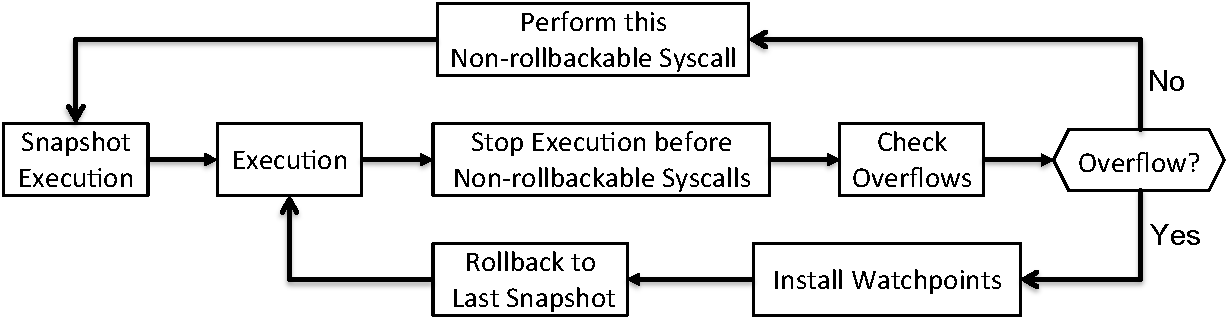
\includegraphics[width=6.5in]{figure/stopgapoverview}
	\caption{\DoubleTake{} diagram. \label{fig:phases}}
	}
\end{figure*}

\subsection{Normal Execution}
\label{sec:normal_execution}

% TODO: Fill in irrevocable system call
\doubletake{} breaks the execution of a program into multiple epochs at irrevocable system calls.
In the beginning of an epoch, \doubletake{} takes a snapshot of the program state. 
During an epoch, \doubletake{} records the program's operations to facilitate re-execution. 
An epoch ends when the program attempts to issue an irrevocable system call, such as \texttt{fork}. 
Before the system call is issued, \doubletake{} checks the program state for errors. 
When no error is detected, \doubletake{} will issue the irrevocable system call and start a new epoch.
If an error is detected, \doubletake{} switches to re-execution mode 
(described in Section~\ref{sec:re-execution}) to gather additional information about memory errors. 

\subsubsection{Starting an Epoch}
{\em Snapshot}. 
At the beginning of every epoch, \doubletake{} take a snapshot of the current program state 
so that we can rollback to this state if there are some errors detected at the end of the current epoch.
A snapshot includes the state of registers (obtained using \texttt{getcontext()}),
and all writable memory, including the globals, the stack and the program heap. 
Read-only memory, such as text segments of a program and libraries, does not need to 
be saved in the snapshot. \doubletake{} analyzes the Linux file \texttt{/proc/self/map} 
to identify the ranges of different memory mappings, including the globals and the stack.
It knows the range of the program heap because of using a customized memory allocator, which is discussed in
Section~\ref{sec:allocator}.  

To snapshot, it first saves the globals of this program and different libraries, 
and then the heap and the stack. 
In the end, it calls \texttt{getcontext} of \texttt{glibc} library to save its execution context.

{\em File Positions}. \doubletake{} records file positions of all opening files
in order to reduce the number of epochs in a program, 
which has been discussed in Section~\ref{sec:syscall}.
For a normal file, \doubletake{} calls \texttt{lseek} to acquire its file position.
For a file opened by \texttt{fopen}-like library calls,
\doubletake{} also saves its corresponding stream additionally.

\subsubsection{Executing an Epoch}
\label{sec:inepoch}
Inside an epoch, \doubletake{} intercepts those library functions involved in system calls 
and handles correspondingly according to the discussion of Section~\ref{sec:syscall}.

For checkpointable system calls, e.g., \texttt{read} and \texttt{write}, since they can 
also be called in socket communications, \doubletake{} has to check whether they 
are working on normal files. In order to speed up the checking process, \doubletake{] is using a hash map to hold file descriptors of all opening files. 
For normal files, reads and writes can be issued normally. 
For reads and writes in network communications, \doubletake{}  ends the current epochs since they are considered to be irrevocable system calls.

For recordable system calls, e.g., \texttt{gettimeofday}, \texttt{time}, and \texttt{mmap},
\doubletake{} records the results of system calls in a First-In-First-Out list, which are necessary to be replayed in re-execution phase if memory errors are detected at the end of the current epoch. 
For \texttt{open}-like library calls, \doubletake{} not only records file descriptors returned by system calls,
but also adds them to the hash map discussed above.  

For delayable system calls, e.g., \texttt{munmap} and \texttt{close}, they are added into a global 
list and are issued in the end of the current epoch after checkings of memory errors.

\subsubsection{Ending an Epoch}
At the end of each epoch, \doubletake{} checks the program state for errors. 
We have implemented error detection for heap buffer overflows (Section~\ref{sec:overflow}), 
memory leakage (Section~\ref{sec:leak}),
and memory use-after-free errors (Section~\ref{sec:danglingpointer}).

When \doubletake{} do not find any memory error, it issues all delayable system calls 
and cleans corresponding lists.
\doubletake{} also cleans recordable system calls
since there is no need to replay those system calls any more.
 
If \doubletake{} finds any memory error, it switches to the re-execution mode, discussed in Section\ref{sec:re-execution}.

\subsection{Rollback and Re-Execution}
\label{sec:re-execution}
When \doubletake{} detects an error, it uses rollback and re-execution to collect additional information to aid programmers in correcting the error. This additional information is either impossible or expensive to collect during normal execution.
In normal execution, it is impossible to know those instructions responsible for buffer overflows and 
memory usage-after-free errors if we do not check every memory access. 
Checking every memory access obviously introduces significant performance overhead, which \doubletake{} avoids. 
It is expensive to acquire call stacks for every memory allocation for detecting memory leakage, \doubletake{} leaves this operation to re-execution phase when memory leakage is detected.
By doing this, \doubletake{} enables programs to run with very low overhead until an error is detected.

\subsubsection*{Preparation}
\doubletake{} does some preparation before it rolls back and re-execute a program with memory errors. 
In order to locate instructions responsible for buffer overflows and memory usage-after-free errors,
\doubletake{} installs watch points on addresses with corrupted canaries, as described in Section~\ref{sec:applications}.
Hardware watch points are configured with debug registers, 
but these registers are only accessible to the kernel. 
Using \texttt{ptrace} function, \doubletake{} forks a child process to install watch points for current process.  

To find the allocation sites and de-allocation sites for memory usage-after-free errors and memory leakage problems, 
\doubletake{} puts all suspected heap objects into a hash map, which are checked for every memory allocation and deallocation. 

Additionally, \doubletake{} calls \texttt{lseek} to recover file positions of all opening files.

\subsubsection*{Rollback}
Regardless of the error detection being used, \doubletake{} must roll back program state 
before the epoch with errors can be re-executed. Before the program stack can be restored, \doubletake{} must switch to a temporary stack since the stack restore process may overwrite its own stack. Next, \doubletake{} restores the state of all writable memory from the epoch's snapshot. Finally, \doubletake{} restores register state with the \texttt{setcontext()} function and re-execution proceeds automatically.

\subsubsection*{Re-Execution}
The main task of re-execution is to collect additional information about different memory errors, which
have been discussed in Section~\ref{sec:applications}. 
In re-execution phase, \doubletake{} repeats the results of recordable system calls by reusing results recorded in normal execution.
For delayable system calls, \doubletake{} turns them to no-op in the re-execution phase.  
